\begin{frame}
    \frametitle{Some experiments with BAliBASE dataset}
    \begin{itemize}
        \item The BAliBASE dataset:
        \begin{itemize}
            \item 141 reference protein alignments.
            \item Hand constructed alignmets from the literature.
            \item 5 subsets with alignments of different characteristics.   
            \item Test alignmets are scored respect \textbf{core blocks} $\rightarrow$ reliable alignmets.         
        \end{itemize}
        \item \textbf{No universally accepted accuracy measure for protein alignmets.}
        \begin{itemize}
            \item Sum-of-pairs score (SP).
            \item Column score (CS).            
        \end{itemize}
    \end{itemize}
\end{frame}

\begin{frame}
    \frametitle{Column reliability for BAliBASE}
    \begin{columns}
        \column{0.5\textwidth}  
            \begin{figure}[t]
                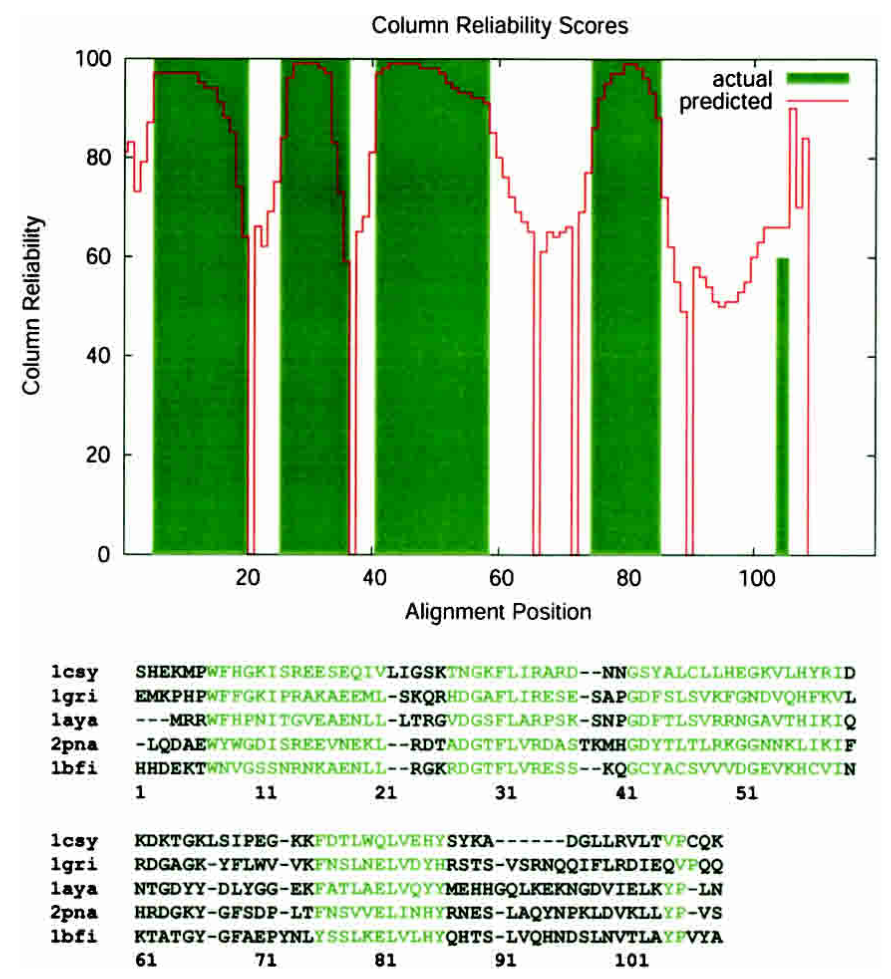
\includegraphics[width=0.6\textheight]{img/exp1.png}
            \end{figure}
        \column{0.47\textwidth}
            \textbf{Image from \cite{do2005probcons}.} 

            At each position:
            \begin{itemize}
                \item Red line $\rightarrow$ predicted proportion of correct pairwise matches.
                \item Green Blocks $\rightarrow$ actual proportion of correct pairwise matches.
            \end{itemize}
    \end{columns}
\end{frame}

\begin{frame}
    \frametitle{Comparison with other methods}
    \begin{figure}[t]
        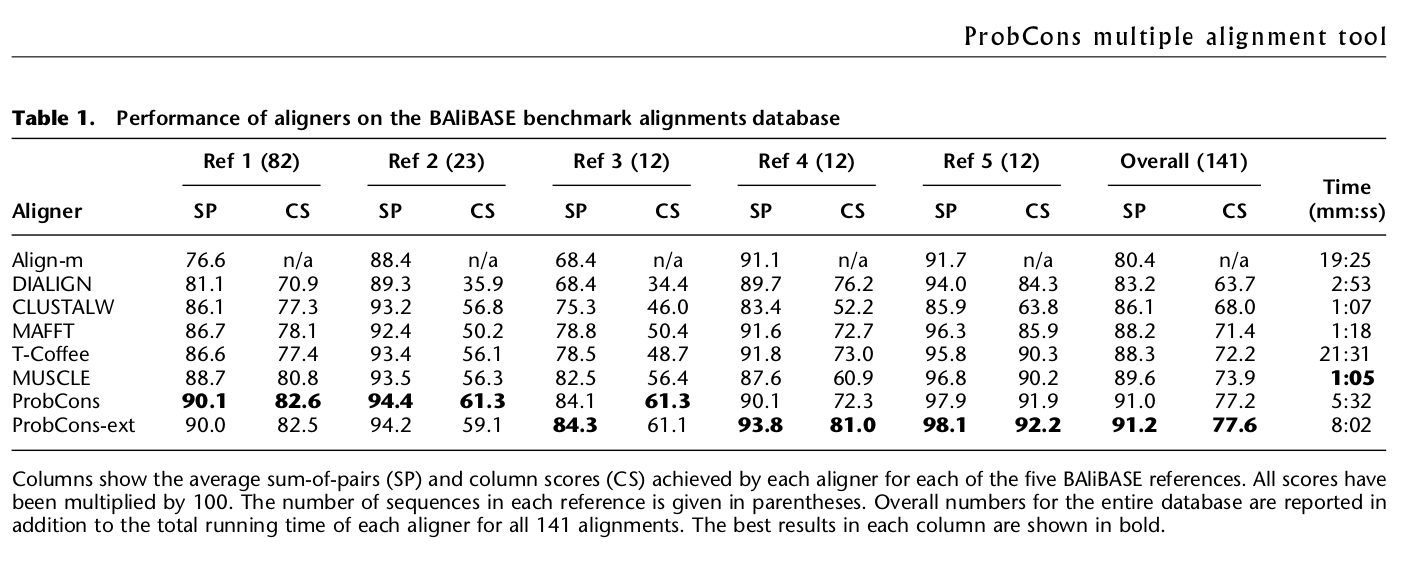
\includegraphics[width=0.9\textwidth]{img/exp2.png}
        \caption{Image from \cite{do2005probcons}.}
    \end{figure}
\end{frame}